\documentclass[t]{beamer}

\usetheme{metropolis}

\usepackage{graphicx}
\usepackage{multirow}
\usepackage{pgfplots}
\usepackage{pgfplotstable}
\usepackage{subcaption}
\usepackage{tikz}
\usepackage{transparent}

\author{Esten H{\o}yland Leonardsen}
\institute[Life Science, UiO]{UiO:Life Science, University of Oslo}
\date{20.10.22}
\title{Detecting individual-level deviations in brain morphology among MCI patients with explainable AI}

\titlegraphic{
	\vspace*{6.8cm}
	\centering
    \includegraphics[width=1.5cm]{data/uio.png}
}
% TIKZ PACKAGES
\usetikzlibrary{arrows.meta}
\usetikzlibrary{calc}
\usetikzlibrary{patterns}
\usetikzlibrary{positioning}
\usetikzlibrary{shapes}

% PGFPLOTS PACKAGES
\usepgfplotslibrary{fillbetween}
\usepgfplotslibrary{groupplots}

% COLOUR
\definecolor{cb-pink}{HTML}{eeafcf}
\definecolor{cb-orange}{HTML}{e59145}
\definecolor{cb-light-brown}{HTML}{baa066}
\definecolor{cb-blue}{HTML}{3594d6}
\definecolor{cb-green}{HTML}{4dac93}
\definecolor{cb-gray}{HTML}{3a5c7d}
\definecolor{cb-light-purple}{HTML}{b45899}
\definecolor{cb-red-purple}{HTML}{c71555}
\definecolor{cb-brown}{HTML}{840000}
\definecolor{cb-blue-purple}{HTML}{662fa2}

\colorlet{cases-default}{cb-red-purple}
\colorlet{controls-default}{cb-blue}
\colorlet{healthy-default}{cb-green}

\definecolor{color0}{rgb}{0.62, 0.004, 0.259}
\definecolor{color1}{rgb}{0.755, 0.154, 0.291}
\definecolor{color2}{rgb}{0.866, 0.29, 0.298}
\definecolor{color3}{rgb}{0.943, 0.406, 0.268}
\definecolor{color4}{rgb}{0.975, 0.557, 0.323}
\definecolor{color5}{rgb}{0.993, 0.709, 0.403}
\definecolor{color6}{rgb}{0.995, 0.832, 0.506}
\definecolor{color7}{rgb}{0.998, 0.926, 0.625}
\definecolor{color8}{rgb}{0.998, 0.999, 0.746}
\definecolor{color9}{rgb}{0.937, 0.975, 0.65}
\definecolor{color10}{rgb}{0.838, 0.935, 0.609}
\definecolor{color11}{rgb}{0.693, 0.876, 0.639}
\definecolor{color12}{rgb}{0.527, 0.811, 0.645}
\definecolor{color13}{rgb}{0.368, 0.725, 0.662}
\definecolor{color14}{rgb}{0.24, 0.582, 0.721}
\definecolor{color15}{rgb}{0.267, 0.441, 0.698}
\definecolor{color16}{rgb}{0.369, 0.31, 0.635}

\pgfplotstableread[col sep=comma]{data/predictions/test_distributions.csv}\testdistributions
\pgfplotstableread[col sep=comma]{data/predictions/test_predictions.csv}\testpredictions
\pgfplotstableread[col sep=comma]{data/predictions/test_auc.csv}\testauc

\begin{document}

	\newcommand{\N}{1}

	\begin{frame}
		\titlepage
	\end{frame}

	{
    	\setbeamertemplate{footline}{\hspace{0.33cm}\hfill \textcolor{gray}{\tiny{\href{https://lrpserver.hhi.fraunhofer.de/image-classification9}{https://lrpserver.hhi.fraunhofer.de/image-classification}}} \hfill \scriptsize{2} \hspace{0.24cm}\vspace{0.4cm}}
		\begin{frame}{Explainable AI} % Nature of explanations
			\centering
			\vfill
			\begin{tikzpicture}
				\node[] at (-5, -5) {};
				\node[] at (-2,1) {
					\includegraphics[width=3cm]{data/ladybug.png}
				};
				\node[] at (2, 1) {
					\includegraphics[width=3cm]{data/ladybug_explanation.png}
				};
				\node[] at (5, 5) {};
			\end{tikzpicture}

			\vfill
		\end{frame}
	}

	\begin{frame}{Overview}
		\begin{figure}
			\def\plotwidth{11.68}

			\newcommand{\nodesize}{11pt}
			\newcommand{\hsep}{28pt}
			\newcommand{\vsep}{14pt}

			\newcommand{\arrowwidth}{0.05cm}
			\newcommand{\innerarrow}{{Latex[length=0.1cm, width=0.15cm]}}
			\newcommand{\outerarrow}{{Latex[length=0.2cm, width=0.3cm]}}

			\definecolor{outercolor}{RGB}{128, 128, 128}
			\colorlet{train-fill}{cb-green}

			\scalebox{0.4}{
				\hspace{3cm}
				\fbox{
					\begin{tikzpicture}
						\newcommand{\mrivsep}{0.52}
						\newcommand{\mrihsep}{0.44}

						\node[anchor=north west] at (0, 0) {\footnotesize{1. Train binary classification CNNs to detect signs of dementia in structural MRIs}};
						\node[anchor=north east] at (\plotwidth, 0) {};

						\newcommand{\patientlocation}[1]{($ (1, -1.6) + ####1 $)}
						\newcommand{\controllocation}[1]{($ (1, -2.8) + ####1 $)}
						\newcommand{\modellocation}[1]{($ (0.5 * \plotwidth, -2.2) + ####1 $)}


						\node[anchor=south, align=center, font=\scriptsize\linespread{0.85}\selectfont] at \patientlocation{(0, 0.48)} {Dementia\\patients};
						\node[anchor=north] at \controllocation{(0, -0.48)} {\scriptsize{Controls}};

						\node[] at \patientlocation{(-1 * \mrihsep, -0.5*\mrivsep)} {
							\includegraphics[height=0.5cm]{data/mris/slice_0.png}
						};
						\node[] at \patientlocation{(0, -0.5*\mrivsep)} {
							\includegraphics[height=0.5cm]{data/mris/slice_1.png}
						};
						\node[] at \patientlocation{(1 * \mrihsep, -0.5*\mrivsep)} {
							\includegraphics[height=0.5cm]{data/mris/slice_2.png}
						};
						\node[] at \patientlocation{(-1 * \mrihsep, 0.5*\mrivsep)} {
							\includegraphics[height=0.5cm]{data/mris/slice_3.png}
						};
						\node[] at \patientlocation{(0, 0.5*\mrivsep)} {
							\includegraphics[height=0.5cm]{data/mris/slice_4.png}
						};
						\node[] at \patientlocation{(1 * \mrihsep, 0.5*\mrivsep)} {
							\includegraphics[height=0.5cm]{data/mris/slice_5.png}
						};

						\node[] at \controllocation{(-1 * \mrihsep, -0.5*\mrivsep)} {
							\includegraphics[height=0.5cm]{data/mris/slice_6.png}
						};
						\node[] at \controllocation{(0, -0.5*\mrivsep)} {
							\includegraphics[height=0.5cm]{data/mris/slice_7.png}
						};
						\node[] at \controllocation{(1 * \mrihsep, -0.5*\mrivsep)} {
							\includegraphics[height=0.5cm]{data/mris/slice_8.png}
						};
						\node[] at \controllocation{(-1 * \mrihsep, 0.5*\mrivsep)} {
							\includegraphics[height=0.5cm]{data/mris/slice_9.png}
						};
						\node[] at \controllocation{(0, 0.5*\mrivsep)} {
							\includegraphics[height=0.5cm]{data/mris/slice_10.png}
						};
						\node[] at \controllocation{(1 * \mrihsep, 0.5*\mrivsep)} {
							\includegraphics[height=0.5cm]{data/mris/slice_11.png}
						};

						\node[circle, inner sep=0pt, fill=none, outer sep=0pt, line width=0pt, draw=none] (n00) at \modellocation{(-3 * \hsep, 0)} {};

						\node[circle, minimum size=\nodesize, inner sep=0pt, fill=train-fill!35, outer sep=0pt, line width=0pt, draw=train-fill!35] (n10) at \modellocation{(-2 * \hsep, 2 * \vsep)} {};
						\node[circle, minimum size=\nodesize, inner sep=0pt, fill=train-fill, outer sep=0pt, line width=0pt, draw=train-fill] (n11) at \modellocation{(-2 * \hsep, 1 * \vsep)} {};
						\node[circle, minimum size=\nodesize, inner sep=0pt, fill=train-fill!15, outer sep=0pt, line width=0pt, draw=train-fill!15] (n12) at \modellocation{(-2 * \hsep, 0)} {};
						\node[circle, minimum size=\nodesize, inner sep=0pt, fill=train-fill!85, outer sep=0pt, line width=0pt, draw=train-fill!85] (n13) at \modellocation{(-2 * \hsep, -1 * \vsep)} {};
						\node[circle, minimum size=\nodesize, inner sep=0pt, fill=train-fill!90, outer sep=0pt, line width=0pt, draw=train-fill!90] (n14) at \modellocation{(-2 * \hsep, -2 * \vsep)} {};

						\node[circle, minimum size=\nodesize, inner sep=0pt, fill=train-fill!55, outer sep=0pt, line width=0pt, draw=train-fill!55] (n20) at \modellocation{(-1 * \hsep, 1.5 * \vsep)} {};
						\node[circle, minimum size=\nodesize, inner sep=0pt, fill=train-fill!20, outer sep=0pt, line width=0pt, draw=train-fill!20] (n21) at \modellocation{(-1 * \hsep, 0.5 * \vsep)} {};
						\node[circle, minimum size=\nodesize, inner sep=0pt, fill=train-fill!90, outer sep=0pt, line width=0pt, draw=train-fill!50] (n22) at \modellocation{(-1 * \hsep, -0.5 * \vsep)} {};
						\node[circle, minimum size=\nodesize, inner sep=0pt, fill=train-fill!35, outer sep=0pt, line width=0pt, draw=train-fill!35] (n23) at \modellocation{(-1 * \hsep, -1.5 * \vsep)} {};

						\node[circle, minimum size=\nodesize, inner sep=0pt, fill=train-fill!95, outer sep=0pt, line width=0pt, draw=train-fill!65] (n30) at \modellocation{(0 * \hsep, 1.5 * \vsep)} {};
						\node[circle, minimum size=\nodesize, inner sep=0pt, fill=train-fill!20, outer sep=0pt, line width=0pt, draw=train-fill!20] (n31) at \modellocation{(0 * \hsep, 0.5 * \vsep)} {};
						\node[circle, minimum size=\nodesize, inner sep=0pt, fill=train-fill!90, outer sep=0pt, line width=0pt, draw=train-fill!90] (n32) at \modellocation{(0 * \hsep, -0.5 * \vsep)} {};
						\node[circle, minimum size=\nodesize, inner sep=0pt, fill=train-fill!80, outer sep=0pt, line width=0pt, draw=train-fill!80] (n33) at \modellocation{(0 * \hsep, -1.5 * \vsep)} {};

						\node[circle, minimum size=\nodesize, inner sep=0pt, fill=train-fill!50, outer sep=0pt, line width=0pt, draw=train-fill!50] (n40) at \modellocation{(1 * \hsep, 1*\vsep)} {};
						\node[circle, minimum size=\nodesize, inner sep=0pt, fill=train-fill!90, outer sep=0pt, line width=0pt, draw=train-fill!70] (n41) at \modellocation{(1 * \hsep, 0*\vsep)} {};
						\node[circle, minimum size=\nodesize, inner sep=0pt, fill=train-fill!70, outer sep=0pt, line width=0pt, draw=train-fill!30] (n42) at \modellocation{(1 * \hsep, -1*\vsep)} {};

						\node[circle, minimum size=\nodesize, inner sep=0pt, fill=train-fill, outer sep=0pt, line width=0pt, draw=train-fill] (n50) at \modellocation{(2 * \hsep, 1*\vsep)} {};
						\node[circle, minimum size=\nodesize, inner sep=0pt, fill=train-fill!70, outer sep=0pt, line width=0pt, draw=train-fill!70] (n51) at \modellocation{(2 * \hsep, 0*\vsep)} {};
						\node[circle, minimum size=\nodesize, inner sep=0pt, fill=train-fill!30, outer sep=0pt, line width=0pt, draw=train-fill!30] (n52) at \modellocation{(2 * \hsep, -1*\vsep)} {};

						\node[circle, minimum size=\nodesize, inner sep=0pt, fill=train-fill!80, outer sep=0pt, line width=0pt, draw=train-fill!65] (n60) at \modellocation{(3 * \hsep, 0)} {};

						\node[] (loss) at (1+2*4.85, -2.2) {\scriptsize{$logloss(y, \hat{y})$}};

						\draw[
							color=train-fill!35,
							\innerarrow-\innerarrow,
							line width=\arrowwidth
						] (n00) to [out=20,in=200] (n10) {};
						\draw[
							color=train-fill,
							\innerarrow-\innerarrow,
							line width=\arrowwidth
						] (n00) to [out=10,in=190] (n11) {};
						\draw[
							color=train-fill!15,
							\innerarrow-\innerarrow,
							line width=\arrowwidth
						] (n00) to [out=0,in=180] (n12) {};
						\draw[
							color=train-fill!85,
							\innerarrow-\innerarrow,
							line width=\arrowwidth
						] (n00) to [out=-10,in=170] (n13) {};
						\draw[
							color=train-fill!90,
							\innerarrow-\innerarrow,
							line width=\arrowwidth
						] (n00) to [out=-20,in=160] (n14) {};

						\draw[
							color=train-fill!35,
							\innerarrow-\innerarrow,
							line width=\arrowwidth
						] (n10) to [out=-5,in=175] (n20) {};
						\draw[
							color=train-fill!10,
							\innerarrow-\innerarrow,
							line width=\arrowwidth
						] (n10) to [out=-15,in=165] (n21) {};
						\draw[
							color=train-fill!70,
							\innerarrow-\innerarrow,
							line width=\arrowwidth
						] (n10) to [out=-25,in=155] (n22) {};
						\draw[
							color=train-fill!50,
							\innerarrow-\innerarrow,
							line width=\arrowwidth
						] (n10) to [out=-35,in=145] (n23) {};

						\draw[
							color=train-fill!30,
							\innerarrow-\innerarrow,
							line width=\arrowwidth
						] (n11) to [out=5,in=185] (n20) {};
						\draw[
							color=train-fill!25,
							\innerarrow-\innerarrow,
							line width=\arrowwidth
						] (n11) to [out=-5,in=175] (n21) {};
						\draw[
							color=train-fill!95,
							\innerarrow-\innerarrow,
							line width=\arrowwidth
						] (n11) to [out=-15,in=165] (n22) {};
						\draw[
							color=train-fill!35,
							\innerarrow-\innerarrow,
							line width=\arrowwidth
						] (n11) to [out=-25,in=155] (n23) {};

						\draw[
							color=train-fill!70,
							\innerarrow-\innerarrow,
							line width=\arrowwidth
						] (n12) to [out=15,in=195] (n20) {};
						\draw[
							color=train-fill!20,
							\innerarrow-\innerarrow,
							line width=\arrowwidth
						] (n12) to [out=5,in=185] (n21) {};
						\draw[
							color=train-fill!80,
							\innerarrow-\innerarrow,
							line width=\arrowwidth
						] (n12) to [out=-5,in=175] (n22) {};
						\draw[
							color=train-fill,
							\innerarrow-\innerarrow,
							line width=\arrowwidth
						] (n12) to [out=-15,in=165] (n23) {};

						\draw[
							color=train-fill!40,
							\innerarrow-\innerarrow,
							line width=\arrowwidth
						] (n13) to [out=25,in=205] (n20) {};
						\draw[
							color=train-fill!35,
							\innerarrow-\innerarrow,
							line width=\arrowwidth
						] (n13) to [out=15,in=195] (n21) {};
						\draw[
							color=train-fill!20,
							\innerarrow-\innerarrow,
							line width=\arrowwidth
						] (n13) to [out=5,in=185] (n22) {};
						\draw[
							color=white,
							\innerarrow-\innerarrow,
							line width=\arrowwidth
						] (n13) to [out=-5,in=175] (n23) {};

						\draw[
							color=train-fill!40,
							\innerarrow-\innerarrow,
							line width=\arrowwidth
						] (n14) to [out=35,in=215] (n20) {};
						\draw[
							color=train-fill!85,
							\innerarrow-\innerarrow,
							line width=\arrowwidth
						] (n14) to [out=25,in=205] (n21) {};
						\draw[
							color=train-fill!35,
							\innerarrow-\innerarrow,
							line width=\arrowwidth
						] (n14) to [out=15,in=195] (n22) {};
						\draw[
							color=train-fill,
							\innerarrow-\innerarrow,
							line width=\arrowwidth
						] (n14) to [out=5,in=185] (n23) {};

						\draw[
							color=train-fill!85,
							\innerarrow-\innerarrow,
							line width=\arrowwidth
						] (n20) to [out=0,in=180] (n30) {};
						\draw[
							color=train-fill!50,
							\innerarrow-\innerarrow,
							line width=\arrowwidth
						] (n20) to [out=-10,in=170] (n31) {};
						\draw[
							color=train-fill!75,
							\innerarrow-\innerarrow,
							line width=\arrowwidth
						] (n20) to [out=-20,in=160] (n32) {};
						\draw[
							color=white,
							\innerarrow-\innerarrow,
							line width=\arrowwidth
						] (n20) to [out=-30,in=150] (n33) {};

						\draw[
							color=train-fill,
							\innerarrow-\innerarrow,
							line width=\arrowwidth
						] (n21) to [out=10,in=190] (n30) {};
						\draw[
							color=train-fill!30,
							\innerarrow-\innerarrow,
							line width=\arrowwidth
						] (n21) to [out=0,in=180] (n31) {};
						\draw[
							color=train-fill!25,
							\innerarrow-\innerarrow,
							line width=\arrowwidth
						] (n21) to [out=-10,in=170] (n32) {};
						\draw[
							color=white,
							\innerarrow-\innerarrow,
							line width=\arrowwidth
						] (n21) to [out=-20,in=160] (n33) {};

						\draw[
							color=train-fill!35,
							\innerarrow-\innerarrow,
							line width=\arrowwidth
						] (n22) to [out=20,in=200] (n30) {};
						\draw[
							color=train-fill!95,
							\innerarrow-\innerarrow,
							line width=\arrowwidth
						] (n22) to [out=10,in=190] (n31) {};
						\draw[
							color=train-fill!80,
							\innerarrow-\innerarrow,
							line width=\arrowwidth
						] (n22) to [out=0,in=180] (n32) {};
						\draw[
							color=white,
							\innerarrow-\innerarrow,
							line width=\arrowwidth
						] (n22) to [out=-10,in=170] (n33) {};

						\draw[
							color=train-fill!45,
							\innerarrow-\innerarrow,
							line width=\arrowwidth
						] (n23) to [out=30,in=210] (n30) {};
						\draw[
							color=train-fill!70,
							\innerarrow-\innerarrow,
							line width=\arrowwidth
						] (n23) to [out=20,in=200] (n31) {};
						\draw[
							color=train-fill!10,
							\innerarrow-\innerarrow,
							line width=\arrowwidth
						] (n23) to [out=10,in=190] (n32) {};
						\draw[
							color=train-fill!20,
							\innerarrow-\innerarrow,
							line width=\arrowwidth
						] (n23) to [out=0,in=180] (n33) {};

						\draw[
							color=train-fill!50,
							\innerarrow-\innerarrow,
							line width=\arrowwidth
						] (n30) to [out=-5,in=175] (n40) {};
						\draw[
							color=train-fill!30,
							\innerarrow-\innerarrow,
							line width=\arrowwidth
						] (n30) to [out=-15,in=165] (n41) {};
						\draw[
							color=train-fill,
							\innerarrow-\innerarrow,
							line width=\arrowwidth
						] (n30) to [out=-25,in=155] (n42) {};

						\draw[
							color=train-fill!45,
							\innerarrow-\innerarrow,
							line width=\arrowwidth
						] (n31) to [out=5,in=185] (n40) {};
						\draw[
							color=train-fill!90,
							\innerarrow-\innerarrow,
							line width=\arrowwidth
						] (n31) to [out=-5,in=175] (n41) {};
						\draw[
							color=train-fill!45,
							\innerarrow-\innerarrow,
							line width=\arrowwidth
						] (n31) to [out=-15,in=165] (n42) {};

						\draw[
							color=train-fill!15,
							\innerarrow-\innerarrow,
							line width=\arrowwidth
						] (n32) to [out=15,in=195] (n40) {};
						\draw[
							color=train-fill!70,
							\innerarrow-\innerarrow,
							line width=\arrowwidth
						] (n32) to [out=5,in=185] (n41) {};
						\draw[
							color=train-fill!50,
							\innerarrow-\innerarrow,
							line width=\arrowwidth
						] (n32) to [out=-5,in=175] (n42) {};

						\draw[
							color=train-fill!40,
							\innerarrow-\innerarrow,
							line width=\arrowwidth
						] (n33) to [out=25,in=205] (n40) {};
						\draw[
							color=train-fill!20,
							\innerarrow-\innerarrow,
							line width=\arrowwidth
						] (n33) to [out=15,in=195] (n41) {};
						\draw[
							color=train-fill!90,
							\innerarrow-\innerarrow,
							line width=\arrowwidth
						] (n33) to [out=5,in=185] (n42) {};

						\draw[
							color=train-fill!25,
							\innerarrow-\innerarrow,
							line width=\arrowwidth
						] (n40) to [out=0,in=180] (n50) {};
						\draw[
							color=train-fill!15,
							\innerarrow-\innerarrow,
							line width=\arrowwidth
						] (n40) to [out=-10,in=170] (n51) {};
						\draw[
							color=train-fill,
							\innerarrow-\innerarrow,
							line width=\arrowwidth
						] (n40) to [out=-20,in=160] (n52) {};

						\draw[
							color=train-fill!35,
							\innerarrow-\innerarrow,
							line width=\arrowwidth
						] (n41) to [out=10,in=190] (n50) {};
						\draw[
							color=train-fill!10,
							\innerarrow-\innerarrow,
							line width=\arrowwidth
						] (n41) to [out=0,in=180] (n51) {};
						\draw[
							color=train-fill!90,
							\innerarrow-\innerarrow,
							line width=\arrowwidth
						] (n41) to [out=-10,in=170] (n52) {};

						\draw[
							color=train-fill!50,
							\innerarrow-\innerarrow,
							line width=\arrowwidth
						] (n42) to [out=20,in=200] (n50) {};
						\draw[
							color=train-fill!40,
							\innerarrow-\innerarrow,
							line width=\arrowwidth
						] (n42) to [out=10,in=190] (n51) {};
						\draw[
							color=train-fill!20,
							\innerarrow-\innerarrow,
							line width=\arrowwidth
						] (n42) to [out=0,in=180] (n52) {};

						\draw[
							color=train-fill!80,
							\innerarrow-\innerarrow,
							line width=\arrowwidth,
						] (n50) to [out=-10,in=170] (n60) {};
						\draw[
							color=train-fill!90,
							\innerarrow-\innerarrow,
							line width=\arrowwidth,
						] (n51) to [out=0,in=180] (n60) {};
						\draw[
							color=train-fill!30,
							\innerarrow-\innerarrow,
							line width=\arrowwidth,
						] (n52) to [out=10,in=190] (n60) {};

						\draw[black] (n00.center) --
									($ (n00) + (0, 2*\vsep+0.5*\nodesize+2pt) $) --
									($ (n00) + (6*\hsep+0.5*\nodesize+2pt, 2*\vsep+0.5*\nodesize+2pt) $) --
									($ (n00) + (6*\hsep+0.5*\nodesize+2pt, -2*\vsep-0.5*\nodesize-2pt) $) --
									($ (n00) + (0, -2*\vsep-0.5*\nodesize-2pt) $) --
									(n00.center);

						\node[] at ($ (n30) + (0, \vsep+0.5*\nodesize) $) {\scriptsize{CNN}};

						\draw[
							color=outercolor,
							-\outerarrow,
							line width=0.1cm
						] \patientlocation{(0.65, 0)} to [out=0,in=180] (n00) {};
						\draw[
							color=outercolor,
							-\outerarrow,
							line width=0.1cm
						] \controllocation{(0.65, 0)} to [out=0,in=180] (n00) {};
						\draw[
							color=outercolor,
							\outerarrow-\outerarrow,
							line width=0.1cm
						] (n60) to [out=0,in=180] (loss) {};
					\end{tikzpicture}
				}
			}
			\newline
			\noindent
			\scalebox{0.4}{
				\hspace{3cm}
				\fbox{
					\begin{tikzpicture}
						\newcommand{\mrivsep}{0.52}
						\newcommand{\mrihsep}{0.44}

						\node[anchor=north west] at (0, 0) {\footnotesize{2. Apply model and LRP to achieve individual-level predictions and heatmaps}};
						\node[anchor=north east] at (\plotwidth, 0) {};

						\newcommand{\mrilocation}[1]{($ (1, -2.2) + ####1 $)}
						\newcommand{\modellocation}[1]{($ (0.5 * \plotwidth, -2.2) + ####1 $)}
						\newcommand{\lrplocation}[1]{($ (0.5 * \plotwidth, -5.2) + ####1 $)}
						\def\maplocation{(1, -5.2)}

						\node[anchor=south, align=center, font=\scriptsize\linespread{0.85}\selectfont] at \mrilocation{(0, 0.99)} {All\\subjects};

						\newcommand{\mrialpha}{0.2}
						\colorlet{predict-fill}{cb-blue}
						\colorlet{lrp-fill}{red}

						\node[] at \mrilocation{(-1 * \mrihsep, -1.5*\mrivsep)} {
							{\transparent{\mrialpha}\includegraphics[height=0.5cm]{data/mris/slice_5.png}}
						};
						\node[] at \mrilocation{(0, -1.5*\mrivsep)} {
							{\transparent{\mrialpha}\includegraphics[height=0.5cm]{data/mris/slice_7.png}}
						};
						\node[] at \mrilocation{(1 * \mrihsep, -1.5*\mrivsep)} {
							{\transparent{\mrialpha}\includegraphics[height=0.5cm]{data/mris/slice_11.png}}
						};
						\node[] at \mrilocation{(-1 * \mrihsep, -0.5*\mrivsep)} {
							{\transparent{\mrialpha}\includegraphics[height=0.5cm]{data/mris/slice_1.png}}
						};
						\node[] at \mrilocation{(0, -0.5*\mrivsep)} {
							{\transparent{\mrialpha}\includegraphics[height=0.5cm]{data/mris/slice_3.png}}
						};
						\node[inner sep=0pt, outer sep=0pt] (input) at \mrilocation{(1 * \mrihsep, -0.5*\mrivsep)} {
							\includegraphics[height=0.5cm]{data/mris/slice_4.png}
						};
						\node[] at \mrilocation{(-1 * \mrihsep, 0.5*\mrivsep)} {
							{\transparent{\mrialpha}\includegraphics[height=0.5cm]{data/mris/slice_2.png}}
						};
						\node[] at \mrilocation{(0, 0.5*\mrivsep)} {
							{\transparent{\mrialpha}\includegraphics[height=0.5cm]{data/mris/slice_0.png}}
						};
						\node[] at \mrilocation{(1 * \mrihsep, 0.5*\mrivsep)} {
							{\transparent{\mrialpha}\includegraphics[height=0.5cm]{data/mris/slice_10.png}}
						};
						\node[] at \mrilocation{(-1 * \mrihsep, 1.5*\mrivsep)} {
							{\transparent{\mrialpha}\includegraphics[height=0.5cm]{data/mris/slice_9.png}}
						};
						\node[] at \mrilocation{(0, 1.5*\mrivsep)} {
							{\transparent{\mrialpha}\includegraphics[height=0.5cm]{data/mris/slice_8.png}}
						};
						\node[] at \mrilocation{(1 * \mrihsep, 1.5*\mrivsep)} {
							{\transparent{\mrialpha}\includegraphics[height=0.5cm]{data/mris/slice_6.png}}
						};

						\node[circle, inner sep=0pt, fill=none, outer sep=0pt, line width=0pt, draw=none] (n00) at \modellocation{(-3 * \hsep, 0)} {};

						\node[circle, minimum size=\nodesize, inner sep=0pt, fill=predict-fill!85, outer sep=0pt, line width=0pt, draw=predict-fill!85] (n10) at \modellocation{(-2 * \hsep, 2 * \vsep)} {};
						\node[circle, minimum size=\nodesize, inner sep=0pt, fill=predict-fill, outer sep=0pt, line width=0pt, draw=predict-fill] (n11) at \modellocation{(-2 * \hsep, 1 * \vsep)} {};
						\node[circle, minimum size=\nodesize, inner sep=0pt, fill=predict-fill!75, outer sep=0pt, line width=0pt, draw=predict-fill!75] (n12) at \modellocation{(-2 * \hsep, 0)} {};
						\node[circle, minimum size=\nodesize, inner sep=0pt, fill=predict-fill!15, outer sep=0pt, line width=0pt, draw=predict-fill!15] (n13) at \modellocation{(-2 * \hsep, -1 * \vsep)} {};
						\node[circle, minimum size=\nodesize, inner sep=0pt, fill=predict-fill!50, outer sep=0pt, line width=0pt, draw=predict-fill!50] (n14) at \modellocation{(-2 * \hsep, -2 * \vsep)} {};

						\node[circle, minimum size=\nodesize, inner sep=0pt, fill=predict-fill!15, outer sep=0pt, line width=0pt, draw=predict-fill!15] (n20) at \modellocation{(-1 * \hsep, 1.5 * \vsep)} {};
						\node[circle, minimum size=\nodesize, inner sep=0pt, fill=predict-fill!65, outer sep=0pt, line width=0pt, draw=predict-fill!65] (n21) at \modellocation{(-1 * \hsep, 0.5 * \vsep)} {};
						\node[circle, minimum size=\nodesize, inner sep=0pt, fill=predict-fill!90, outer sep=0pt, line width=0pt, draw=predict-fill!90] (n22) at \modellocation{(-1 * \hsep, -0.5 * \vsep)} {};
						\node[circle, minimum size=\nodesize, inner sep=0pt, fill=predict-fill!40, outer sep=0pt, line width=0pt, draw=predict-fill!40] (n23) at \modellocation{(-1 * \hsep, -1.5 * \vsep)} {};

						\node[circle, minimum size=\nodesize, inner sep=0pt, fill=predict-fill!80, outer sep=0pt, line width=0pt, draw=predict-fill!80] (n30) at \modellocation{(0 * \hsep, 1.5 * \vsep)} {};
						\node[circle, minimum size=\nodesize, inner sep=0pt, fill=predict-fill!55, outer sep=0pt, line width=0pt, draw=predict-fill!55] (n31) at \modellocation{(0 * \hsep, 0.5 * \vsep)} {};
						\node[circle, minimum size=\nodesize, inner sep=0pt, fill=predict-fill!15, outer sep=0pt, line width=0pt, draw=predict-fill!15] (n32) at \modellocation{(0 * \hsep, -0.5 * \vsep)} {};
						\node[circle, minimum size=\nodesize, inner sep=0pt, fill=predict-fill!75, outer sep=0pt, line width=0pt, draw=predict-fill!75] (n33) at \modellocation{(0 * \hsep, -1.5 * \vsep)} {};

						\node[circle, minimum size=\nodesize, inner sep=0pt, fill=predict-fill, outer sep=0pt, line width=0pt, draw=predict-fill] (n40) at \modellocation{(1 * \hsep, 1*\vsep)} {};
						\node[circle, minimum size=\nodesize, inner sep=0pt, fill=predict-fill!20, outer sep=0pt, line width=0pt, draw=predict-fill!20] (n41) at \modellocation{(1 * \hsep, 0*\vsep)} {};
						\node[circle, minimum size=\nodesize, inner sep=0pt, fill=predict-fill!15, outer sep=0pt, line width=0pt, draw=predict-fill!15] (n42) at \modellocation{(1 * \hsep, -1*\vsep)} {};

						\node[circle, minimum size=\nodesize, inner sep=0pt, fill=predict-fill!75, outer sep=0pt, line width=0pt, draw=predict-fill!75] (n50) at \modellocation{(2 * \hsep, 1*\vsep)} {};
						\node[circle, minimum size=\nodesize, inner sep=0pt, fill=predict-fill!35, outer sep=0pt, line width=0pt, draw=predict-fill!35] (n51) at \modellocation{(2 * \hsep, 0*\vsep)} {};
						\node[circle, minimum size=\nodesize, inner sep=0pt, fill=predict-fill!65, outer sep=0pt, line width=0pt, draw=predict-fill!65] (n52) at \modellocation{(2 * \hsep, -1*\vsep)} {};

						\node[circle, minimum size=\nodesize, inner sep=0pt, fill=predict-fill!85, outer sep=0pt, line width=0pt, draw=predict-fill!85] (output) at \modellocation{(3 * \hsep, 0)} {};

						\node[] (diagnosis) at (1+2*4.85, -2.2) {\scriptsize{$\widehat{diagnosis}$}};

						\draw[
							color=predict-fill!85,
							-\innerarrow,
							line width=\arrowwidth
						] (n00) to [out=20,in=200] (n10) {};
						\draw[
							color=predict-fill,
							-\innerarrow,
							line width=\arrowwidth
						] (n00) to [out=10,in=190] (n11) {};
						\draw[
							color=predict-fill!75,
							-\innerarrow,
							line width=\arrowwidth
						] (n00) to [out=0,in=180] (n12) {};
						\draw[
							color=predict-fill!15,
							-\innerarrow,
							line width=\arrowwidth
						] (n00) to [out=-10,in=170] (n13) {};
						\draw[
							color=predict-fill!50,
							-\innerarrow,
							line width=\arrowwidth
						] (n00) to [out=-20,in=160] (n14) {};

						\draw[
							color=predict-fill!75,
							-\innerarrow,
							line width=\arrowwidth
						] (n10) to [out=-5,in=175] (n20) {};
						\draw[
							color=predict-fill!50,
							-\innerarrow,
							line width=\arrowwidth
						] (n10) to [out=-15,in=165] (n21) {};
						\draw[
							color=predict-fill!55,
							-\innerarrow,
							line width=\arrowwidth
						] (n10) to [out=-25,in=155] (n22) {};
						\draw[
							color=predict-fill!85,
							-\innerarrow,
							line width=\arrowwidth
						] (n10) to [out=-35,in=145] (n23) {};

						\draw[
							color=predict-fill!45,
							-\innerarrow,
							line width=\arrowwidth
						] (n11) to [out=5,in=185] (n20) {};
						\draw[
							color=predict-fill!50,
							-\innerarrow,
							line width=\arrowwidth
						] (n11) to [out=-5,in=175] (n21) {};
						\draw[
							color=predict-fill,
							-\innerarrow,
							line width=\arrowwidth
						] (n11) to [out=-15,in=165] (n22) {};
						\draw[
							color=predict-fill!15,
							-\innerarrow,
							line width=\arrowwidth
						] (n11) to [out=-25,in=155] (n23) {};

						\draw[
							color=predict-fill!35,
							-\innerarrow,
							line width=\arrowwidth
						] (n12) to [out=15,in=195] (n20) {};
						\draw[
							color=predict-fill!90,
							-\innerarrow,
							line width=\arrowwidth
						] (n12) to [out=5,in=185] (n21) {};
						\draw[
							color=predict-fill!80,
							-\innerarrow,
							line width=\arrowwidth
						] (n12) to [out=-5,in=175] (n22) {};
						\draw[
							color=predict-fill!20,
							-\innerarrow,
							line width=\arrowwidth
						] (n12) to [out=-15,in=165] (n23) {};

						\draw[
							color=predict-fill!55,
							-\innerarrow,
							line width=\arrowwidth
						] (n13) to [out=25,in=205] (n20) {};
						\draw[
							color=predict-fill!65,
							-\innerarrow,
							line width=\arrowwidth
						] (n13) to [out=15,in=195] (n21) {};
						\draw[
							color=predict-fill!35,
							-\innerarrow,
							line width=\arrowwidth
						] (n13) to [out=5,in=185] (n22) {};
						\draw[
							color=predict-fill!45,
							-\innerarrow,
							line width=\arrowwidth
						] (n13) to [out=-5,in=175] (n23) {};

						\draw[
							color=predict-fill!10,
							-\innerarrow,
							line width=\arrowwidth
						] (n14) to [out=35,in=215] (n20) {};
						\draw[
							color=predict-fill!90,
							-\innerarrow,
							line width=\arrowwidth
						] (n14) to [out=25,in=205] (n21) {};
						\draw[
							color=predict-fill!80,
							-\innerarrow,
							line width=\arrowwidth
						] (n14) to [out=15,in=195] (n22) {};
						\draw[
							color=predict-fill!35,
							-\innerarrow,
							line width=\arrowwidth
						] (n14) to [out=5,in=185] (n23) {};

						\draw[
							color=predict-fill!75,
							-\innerarrow,
							line width=\arrowwidth
						] (n20) to [out=0,in=180] (n30) {};
						\draw[
							color=predict-fill!50,
							-\innerarrow,
							line width=\arrowwidth
						] (n20) to [out=-10,in=170] (n31) {};
						\draw[
							color=predict-fill!85,
							-\innerarrow,
							line width=\arrowwidth
						] (n20) to [out=-20,in=160] (n32) {};
						\draw[
							color=predict-fill!45,
							-\innerarrow,
							line width=\arrowwidth
						] (n20) to [out=-30,in=150] (n33) {};

						\draw[
							color=predict-fill!20,
							-\innerarrow,
							line width=\arrowwidth
						] (n21) to [out=10,in=190] (n30) {};
						\draw[
							color=predict-fill!35,
							-\innerarrow,
							line width=\arrowwidth
						] (n21) to [out=0,in=180] (n31) {};
						\draw[
							color=predict-fill!15,
							-\innerarrow,
							line width=\arrowwidth
						] (n21) to [out=-10,in=170] (n32) {};
						\draw[
							color=predict-fill!90,
							-\innerarrow,
							line width=\arrowwidth
						] (n21) to [out=-20,in=160] (n33) {};

						\draw[
							color=predict-fill!65,
							-\innerarrow,
							line width=\arrowwidth
						] (n22) to [out=20,in=200] (n30) {};
						\draw[
							color=predict-fill!20,
							-\innerarrow,
							line width=\arrowwidth
						] (n22) to [out=10,in=190] (n31) {};
						\draw[
							color=predict-fill!30,
							-\innerarrow,
							line width=\arrowwidth
						] (n22) to [out=0,in=180] (n32) {};
						\draw[
							color=predict-fill!40,
							-\innerarrow,
							line width=\arrowwidth
						] (n22) to [out=-10,in=170] (n33) {};

						\draw[
							color=predict-fill,
							-\innerarrow,
							line width=\arrowwidth
						] (n23) to [out=30,in=210] (n30) {};
						\draw[
							color=predict-fill!15,
							-\innerarrow,
							line width=\arrowwidth
						] (n23) to [out=20,in=200] (n31) {};
						\draw[
							color=predict-fill!75,
							-\innerarrow,
							line width=\arrowwidth
						] (n23) to [out=10,in=190] (n32) {};
						\draw[
							color=predict-fill!35,
							-\innerarrow,
							line width=\arrowwidth
						] (n23) to [out=0,in=180] (n33) {};

						\draw[
							color=predict-fill!70,
							-\innerarrow,
							line width=\arrowwidth
						] (n30) to [out=-5,in=175] (n40) {};
						\draw[
							color=predict-fill!80,
							-\innerarrow,
							line width=\arrowwidth
						] (n30) to [out=-15,in=165] (n41) {};
						\draw[
							color=predict-fill!20,
							-\innerarrow,
							line width=\arrowwidth
						] (n30) to [out=-25,in=155] (n42) {};

						\draw[
							color=predict-fill!60,
							-\innerarrow,
							line width=\arrowwidth
						] (n31) to [out=5,in=185] (n40) {};
						\draw[
							color=predict-fill!95,
							-\innerarrow,
							line width=\arrowwidth
						] (n31) to [out=-5,in=175] (n41) {};
						\draw[
							color=predict-fill!35,
							-\innerarrow,
							line width=\arrowwidth
						] (n31) to [out=-15,in=165] (n42) {};

						\draw[
							color=predict-fill!75,
							-\innerarrow,
							line width=\arrowwidth
						] (n32) to [out=15,in=195] (n40) {};
						\draw[
							color=predict-fill!20,
							-\innerarrow,
							line width=\arrowwidth
						] (n32) to [out=5,in=185] (n41) {};
						\draw[
							color=predict-fill!15,
							-\innerarrow,
							line width=\arrowwidth
						] (n32) to [out=-5,in=175] (n42) {};

						\draw[
							color=predict-fill!40,
							-\innerarrow,
							line width=\arrowwidth
						] (n33) to [out=25,in=205] (n40) {};
						\draw[
							color=predict-fill!80,
							-\innerarrow,
							line width=\arrowwidth
						] (n33) to [out=15,in=195] (n41) {};
						\draw[
							color=predict-fill!50,
							-\innerarrow,
							line width=\arrowwidth
						] (n33) to [out=5,in=185] (n42) {};

						\draw[
							color=predict-fill!25,
							-\innerarrow,
							line width=\arrowwidth
						] (n40) to [out=0,in=180] (n50) {};
						\draw[
							color=predict-fill!50,
							-\innerarrow,
							line width=\arrowwidth
						] (n40) to [out=-10,in=170] (n51) {};
						\draw[
							color=predict-fill!45,
							-\innerarrow,
							line width=\arrowwidth
						] (n40) to [out=-20,in=160] (n52) {};

						\draw[
							color=predict-fill!90,
							-\innerarrow,
							line width=\arrowwidth
						] (n41) to [out=10,in=190] (n50) {};
						\draw[
							color=predict-fill!10,
							-\innerarrow,
							line width=\arrowwidth
						] (n41) to [out=0,in=180] (n51) {};
						\draw[
							color=predict-fill!75,
							-\innerarrow,
							line width=\arrowwidth
						] (n41) to [out=-10,in=170] (n52) {};

						\draw[
							color=predict-fill!60,
							-\innerarrow,
							line width=\arrowwidth
						] (n42) to [out=20,in=200] (n50) {};
						\draw[
							color=predict-fill!25,
							-\innerarrow,
							line width=\arrowwidth
						] (n42) to [out=10,in=190] (n51) {};
						\draw[
							color=predict-fill!15,
							-\innerarrow,
							line width=\arrowwidth
						] (n42) to [out=0,in=180] (n52) {};

						\draw[
							color=predict-fill!95,
							-\innerarrow,
							line width=\arrowwidth
						] (n50) to [out=-10,in=170] (output) {};
						\draw[
							color=predict-fill!25,
							-\innerarrow,
							line width=\arrowwidth
						] (n51) to [out=0,in=180] (output) {};
						\draw[
							color=predict-fill!50,
							-\innerarrow,
							line width=\arrowwidth
						] (n52) to [out=10,in=190] (output) {};

						\draw[black] (n00.center) --
									($ (n00) + (0, 2*\vsep+0.5*\nodesize+2pt) $) --
									($ (n00) + (6*\hsep+0.5*\nodesize+2pt, 2*\vsep+0.5*\nodesize+2pt) $) --
									($ (n00) + (6*\hsep+0.5*\nodesize+2pt, -2*\vsep-0.5*\nodesize-2pt) $) --
									($ (n00) + (0, -2*\vsep-0.5*\nodesize-2pt) $) -- (n00.center);

						\node[] at ($ (n30) + (0, \vsep+0.5*\nodesize) $) {\footnotesize{CNN}};

						\draw[
							color=outercolor,
							-\outerarrow,
							line width=0.1cm
						] (input) to [out=0,in=180] (n00) {};
						\draw[
							color=outercolor,
							-\outerarrow,
							line width=0.1cm
						] (output) to [out=0,in=180] (diagnosis) {};

						\node[circle, inner sep=0pt, fill=none, outer sep=0pt, line width=0pt, draw=none] (n00) at \lrplocation{(-3 * \hsep, 0)} {};

						\node[circle, minimum size=\nodesize, inner sep=0pt, fill={rgb:black,5;orange,1}, outer sep=0pt, line width=0pt, draw={rgb:black,5;orange,1}] (n10) at \lrplocation{(-2 * \hsep, 2 * \vsep)} {};
						\node[circle, minimum size=\nodesize, inner sep=0pt, fill={rgb:black,3;red,1}, outer sep=0pt, line width=0pt, draw={rgb:black,3;red,1}] (n11) at \lrplocation{(-2 * \hsep, 1 * \vsep)} {};
						\node[circle, minimum size=\nodesize, inner sep=0pt, fill=yellow, outer sep=0pt, line width=0pt, draw=yellow] (n12) at \lrplocation{(-2 * \hsep, 0)} {};
						\node[circle, minimum size=\nodesize, inner sep=0pt, fill=black, outer sep=0pt, line width=0pt, draw=black] (n13) at \lrplocation{(-2 * \hsep, -1 * \vsep)} {};
						\node[circle, minimum size=\nodesize, inner sep=0pt, fill=red, outer sep=0pt, line width=0pt, draw=red] (n14) at \lrplocation{(-2 * \hsep, -2 * \vsep)} {};

						\node[circle, minimum size=\nodesize, inner sep=0pt, fill={rgb:black,5;white,2;orange,1}, outer sep=0pt, line width=0pt, draw={rgb:black,5;white,2;orange,1}] (n20) at \lrplocation{(-1 * \hsep, 1.5 * \vsep)} {};
						\node[circle, minimum size=\nodesize, inner sep=0pt, fill={rgb:red,10;yellow,6}, outer sep=0pt, line width=0pt, draw={rgb:red,10;yellow,4}] (n21) at \lrplocation{(-1 * \hsep, 0.5 * \vsep)} {};
						\node[circle, minimum size=\nodesize, inner sep=0pt, fill={rgb:red,10;yellow,1}, outer sep=0pt, line width=0pt, draw={rgb:red,10;yellow,1}] (n22) at \lrplocation{(-1 * \hsep, -0.5 * \vsep)} {};
						\node[circle, minimum size=\nodesize, inner sep=0pt, fill={rgb:black,10;red,2}, outer sep=0pt, line width=0pt, draw={rgb:black,10;red,2}] (n23) at \lrplocation{(-1 * \hsep, -1.5 * \vsep)} {};

						\node[circle, minimum size=\nodesize, inner sep=0pt, fill={rgb:red,3;orange,2}, outer sep=0pt, line width=0pt, draw={rgb:red,3;orange,1}] (n30) at \lrplocation{(0 * \hsep, 1.5 * \vsep)} {};
						\node[circle, minimum size=\nodesize, inner sep=0pt, fill={rgb:yellow,3;orange,1}, outer sep=0pt, line width=0pt, draw={rgb:yellow,3;orange,1}] (n31) at \lrplocation{(0 * \hsep, 0.5 * \vsep)} {};
						\node[circle, minimum size=\nodesize, inner sep=0pt, fill={rgb:black,10;white,5;red,1}, outer sep=0pt, line width=0pt, draw={rgb:black,10;white,5;red,1}] (n32) at \lrplocation{(0 * \hsep, -0.5 * \vsep)} {};
						\node[circle, minimum size=\nodesize, inner sep=0pt, fill={rgb:gray,5;red,1}, outer sep=0pt, line width=0pt, draw={rgb:gray,5;red,1}] (n33) at \lrplocation{(0 * \hsep, -1.5 * \vsep)} {};

						\node[circle, minimum size=\nodesize, inner sep=0pt, fill={rgb:yellow,10;orange,1}, outer sep=0pt, line width=0pt, draw={rgb:yellow,10;orange,1}] (n40) at \lrplocation{(1 * \hsep, 1*\vsep)} {};
						\node[circle, minimum size=\nodesize, inner sep=0pt, fill={rgb:red,1}, outer sep=0pt, line width=0pt, draw={rgb:red,1}] (n41) at \lrplocation{(1 * \hsep, 0*\vsep)} {};
						\node[circle, minimum size=\nodesize, inner sep=0pt, fill={rgb:black,10;white,15;red,2}, outer sep=0pt, line width=0pt, draw={rgb:black,10;white,15;red,2}] (n42) at \lrplocation{(1 * \hsep, -1*\vsep)} {};

						\node[circle, minimum size=\nodesize, inner sep=0pt, fill={rgb:red,5;black,1;yellow,2}, outer sep=0pt, line width=0pt, draw={rgb:red,5;black,1;yellow,2}] (n50) at \lrplocation{(2 * \hsep, 1*\vsep)} {};
						\node[circle, minimum size=\nodesize, inner sep=0pt, fill={rgb:gray,5;red,1}, outer sep=0pt, line width=0pt, draw={rgb:gray,5;red,1}] (n51) at \lrplocation{(2 * \hsep, 0*\vsep)} {};
						\node[circle, minimum size=\nodesize, inner sep=0pt, fill={rgb:yellow,5;orange,1}, outer sep=0pt, line width=0pt, draw={rgb:yellow,5;orange,1}] (n52) at \lrplocation{(2 * \hsep, -1*\vsep)} {};

						\node[circle, minimum size=\nodesize, inner sep=0pt, fill={rgb:orange,7;yellow,4;black,1}, outer sep=0pt, line width=0pt, draw={rgb:orange,7;yellow,4;black,1}] (n60) at \lrplocation{(3 * \hsep, 0)} {};

						\draw[
							color={rgb:black,5;orange,1},
							\innerarrow-,
							line width=\arrowwidth
						] (n00) to [out=20,in=200] (n10) {};
						\draw[
							color={rgb:black,3;red,1},
							\innerarrow-,
							line width=\arrowwidth
						] (n00) to [out=10,in=190] (n11) {};
						\draw[
							color=yellow,
							\innerarrow-,
							line width=\arrowwidth
						] (n00) to [out=0,in=180] (n12) {};
						\draw[
							color=black,
							\innerarrow-,
							line width=\arrowwidth
						] (n00) to [out=-10,in=170] (n13) {};
						\draw[
							color=red,
							\innerarrow-,
							line width=\arrowwidth
						] (n00) to [out=-20,in=160] (n14) {};

						\draw[
							color={rgb:black,5;white,1;orange,1},
							\innerarrow-,
							line width=\arrowwidth
						] (n10) to [out=-5,in=175] (n20) {};
						\draw[
							color={rgb:black,3;orange,1},
							\innerarrow-,
							line width=\arrowwidth
						] (n10) to [out=-15,in=165] (n21) {};
						\draw[
							color={rgb:black,4;red,2;yellow,1},
							\innerarrow-,
							line width=\arrowwidth
						] (n10) to [out=-25,in=155] (n22) {};
						\draw[
							color={rgb:black,3;red,1},
							\innerarrow-,
							line width=\arrowwidth
						] (n10) to [out=-35,in=145] (n23) {};

						\draw[
							color={rgb:black,10;orange,2},
							\innerarrow-,
							line width=\arrowwidth
						] (n11) to [out=5,in=185] (n20) {};
						\draw[
							color={rgb:black,3;orange,1},
							\innerarrow-,
							line width=\arrowwidth
						] (n11) to [out=-5,in=175] (n21) {};
						\draw[
							color={rgb:black,3;red,1},
							\innerarrow-,
							line width=\arrowwidth
						] (n11) to [out=-15,in=165] (n22) {};
						\draw[
							color={rgb:black,10;red,1},
							\innerarrow-,
							line width=\arrowwidth
						] (n11) to [out=-25,in=155] (n23) {};

						\draw[
							color={rgb:black,5;orange,3},
							\innerarrow-,
							line width=\arrowwidth
						] (n12) to [out=15,in=195] (n20) {};
						\draw[
							color={rgb:red,3;yellow,5},
							\innerarrow-,
							line width=\arrowwidth
						] (n12) to [out=5,in=185] (n21) {};
						\draw[
							color={rgb:red,5;yellow,3},
							\innerarrow-,
							line width=\arrowwidth
						] (n12) to [out=-5,in=175] (n22) {};
						\draw[
							color={rgb:black,5;orange,2},
							\innerarrow-,
							line width=\arrowwidth
						] (n12) to [out=-15,in=165] (n23) {};

						\draw[
							color={rgb:black,5;red,1},
							\innerarrow-,
							line width=\arrowwidth
						] (n13) to [out=25,in=205] (n20) {};
						\draw[
							color={rgb:black,5;orange,2},
							\innerarrow-,
							line width=\arrowwidth
						] (n13) to [out=15,in=195] (n21) {};
						\draw[
							color={rgb:black,5;red,3},
							\innerarrow-,
							line width=\arrowwidth
						] (n13) to [out=5,in=185] (n22) {};
						\draw[
							color=black,
							\innerarrow-,
							line width=\arrowwidth
						] (n13) to [out=-5,in=175] (n23) {};

						\draw[
							color={rgb:black,5;orange,2},
							\innerarrow-,
							line width=\arrowwidth
						] (n14) to [out=35,in=215] (n20) {};
						\draw[
							color={rgb:red,3;orange,1},
							\innerarrow-,
							line width=\arrowwidth
						] (n14) to [out=25,in=205] (n21) {};
						\draw[
							color={rgb:red,5;yellow,2},
							\innerarrow-,
							line width=\arrowwidth
						] (n14) to [out=15,in=195] (n22) {};
						\draw[
							color={rgb:black,5;red,3},
							\innerarrow-,
							line width=\arrowwidth
						] (n14) to [out=5,in=185] (n23) {};

						\draw[
							color={rgb:black,1;red,1},
							\innerarrow-,
							line width=\arrowwidth
						] (n20) to [out=0,in=180] (n30) {};
						\draw[
							color={rgb:black,3;orange,1},
							\innerarrow-,
							line width=\arrowwidth
						] (n20) to [out=-10,in=170] (n31) {};
						\draw[
							color={rgb:black,10;red,1},
							\innerarrow-,
							line width=\arrowwidth
						] (n20) to [out=-20,in=160] (n32) {};
						\draw[
							color={rgb:black,5;red,1},
							\innerarrow-,
							line width=\arrowwidth
						] (n20) to [out=-30,in=150] (n33) {};

						\draw[
							color={rgb:orange,5;red,2},
							\innerarrow-,
							line width=\arrowwidth
						] (n21) to [out=10,in=190] (n30) {};
						\draw[
							color={rgb:yellow,10;orange,4},
							\innerarrow-,
							line width=\arrowwidth
						] (n21) to [out=0,in=180] (n31) {};
						\draw[
							color={rgb:black,2;red,1},
							\innerarrow-,
							line width=\arrowwidth
						] (n21) to [out=-10,in=170] (n32) {};
						\draw[
							color={rgb:black,1;orange,2;red,1},
							\innerarrow-,
							line width=\arrowwidth
						] (n21) to [out=-20,in=160] (n33) {};

						\draw[
							color={rgb:red,2;orange,1},
							\innerarrow-,
							line width=\arrowwidth
						] (n22) to [out=20,in=200] (n30) {};
						\draw[
							color={rgb:yellow,2;orange,1},
							\innerarrow-,
							line width=\arrowwidth
						] (n22) to [out=10,in=190] (n31) {};
						\draw[
							color={rgb:black,2;red,2},
							\innerarrow-,
							line width=\arrowwidth
						] (n22) to [out=0,in=180] (n32) {};
						\draw[
							color={rgb:black,2;orange,1},
							\innerarrow-,
							line width=\arrowwidth
						] (n22) to [out=-10,in=170] (n33) {};

						\draw[
							color={rgb:black,4;red,2},
							\innerarrow-,
							line width=\arrowwidth
						] (n23) to [out=30,in=210] (n30) {};
						\draw[
							color={rgb:orange,2;black,1},
							\innerarrow-,
							line width=\arrowwidth
						] (n23) to [out=20,in=200] (n31) {};
						\draw[
							color={rgb:black,5;orange,1},
							\innerarrow-,
							line width=\arrowwidth
						] (n23) to [out=10,in=190] (n32) {};
						\draw[
							color={rgb:black,5;red,2},
							\innerarrow-,
							line width=\arrowwidth
						] (n23) to [out=0,in=180] (n33) {};

						\draw[
							color={rgb:orange,3;red,1},
							\innerarrow-,
							line width=\arrowwidth
						] (n30) to [out=-5,in=175] (n40) {};
						\draw[
							color={rgb:gray,1;orange,1;red,2},
							\innerarrow-,
							line width=\arrowwidth
						] (n30) to [out=-15,in=165] (n41) {};
						\draw[
							color={rgb:orange,2;black,2;white,1},
							\innerarrow-,
							line width=\arrowwidth
						] (n30) to [out=-25,in=155] (n42) {};

						\draw[
							color={rgb:yellow,5;orange,1},
							\innerarrow-,
							line width=\arrowwidth
						] (n31) to [out=5,in=185] (n40) {};
						\draw[
							color={rgb:red,3;orange,1},
							\innerarrow-,
							line width=\arrowwidth
						] (n31) to [out=-5,in=175] (n41) {};
						\draw[
							color={rgb:gray,1;red,2},
							\innerarrow-,
							line width=\arrowwidth
						] (n31) to [out=-15,in=165] (n42) {};

						\draw[
							color={rgb:gray,3;orange,1},
							\innerarrow-,
							line width=\arrowwidth
						] (n32) to [out=15,in=195] (n40) {};
						\draw[
							color={rgb:gray,1;red,1},
							\innerarrow-,
							line width=\arrowwidth
						] (n32) to [out=5,in=185] (n41) {};
						\draw[
							color={rgb:gray,1},
							\innerarrow-,
							line width=\arrowwidth
						] (n32) to [out=-5,in=175] (n42) {};

						\draw[
							color={rgb:gray,2;orange,3},
							\innerarrow-,
							line width=\arrowwidth
						] (n33) to [out=25,in=205] (n40) {};
						\draw[
							color={rgb:gray,1;orange,1},
							\innerarrow-,
							line width=\arrowwidth
						] (n33) to [out=15,in=195] (n41) {};
						\draw[
							color={rgb:gray,3;red,1},
							\innerarrow-,
							line width=\arrowwidth
						] (n33) to [out=5,in=185] (n42) {};

						\draw[
							color={rgb:red,3;yellow,1},
							\innerarrow-,
							line width=\arrowwidth
						] (n40) to [out=0,in=180] (n50) {};
						\draw[
							color={rgb:gray,2;orange,1},
							\innerarrow-,
							line width=\arrowwidth
						] (n40) to [out=-10,in=170] (n51) {};
						\draw[
							color={rgb:yellow,10;orange,1},
							\innerarrow-,
							line width=\arrowwidth
						] (n40) to [out=-20,in=160] (n52) {};

						\draw[
							color={rgb:red,5;black,1;yellow,2},
							\innerarrow-,
							line width=\arrowwidth
						] (n41) to [out=10,in=190] (n50) {};
						\draw[
							color={rgb:gray,7;orange,3},
							\innerarrow-,
							line width=\arrowwidth
						] (n41) to [out=0,in=180] (n51) {};
						\draw[
							color={rgb:yellow,1;orange,2},
							\innerarrow-,
							line width=\arrowwidth
						] (n41) to [out=-10,in=170] (n52) {};

						\draw[
							color={rgb:gray,7;orange,2},
							\innerarrow-,
							line width=\arrowwidth
						] (n42) to [out=20,in=200] (n50) {};
						\draw[
							color={rgb:gray,5;red,1},
							\innerarrow-,
							line width=\arrowwidth
						] (n42) to [out=10,in=190] (n51) {};
						\draw[
							color={rgb:gray,5;red,1;black,2},
							\innerarrow-,
							line width=\arrowwidth
						] (n42) to [out=0,in=180] (n52) {};

						\draw[
							color={rgb:red,5;black,1;yellow,2},
							\innerarrow-,
							line width=\arrowwidth
						] (n50) to [out=-10,in=170] (n60) {};
						\draw[
							color={rgb:gray,5;red,1},
							\innerarrow-,
							line width=\arrowwidth
						] (n51) to [out=0,in=180] (n60) {};
						\draw[
							color={rgb:yellow,5;orange,1},
							\innerarrow-,
							line width=\arrowwidth
						] (n52) to [out=10,in=190] (n60) {};

						\draw[black, dashed] (n00.center) --
									($ (n00) + (0, 2*\vsep+0.5*\nodesize+2pt) $) --
									($ (n00) + (6*\hsep+0.5*\nodesize+2pt, 2*\vsep+0.5*\nodesize+2pt) $) --
									($ (n00) + (6*\hsep+0.5*\nodesize+2pt, -2*\vsep-0.5*\nodesize-2pt) $) --
									($ (n00) + (0, -2*\vsep-0.5*\nodesize-2pt) $) -- (n00.center);

						\node[] at ($ (n33) + (0, -1 * \vsep-0.5*\nodesize) $) {\scriptsize{LRP}};

						\draw[double distance=4pt, {Stealth[width=10pt,length=5pt]}-{Stealth[width=10pt,length=5pt]}, line width=1pt] \lrplocation{(0, 2*\vsep+0.5*\nodesize+2pt)} -- \modellocation{(0, -2*\vsep-0.5*\nodesize-2pt)};


						\draw[
							color=outercolor,
							-\outerarrow,
							line width=0.1cm
						] (output) to [out=270,in=90] (n60) {};

						\node[inner sep=0pt, outer sep=0pt,label={[align=center,font=\scriptsize\linespread{0.85}\selectfont]below:\textit{Relevance}\\ \textit{map}}] (map) at \maplocation {
							\includegraphics[
								width=1cm,
								clip=true,
								trim = 128mm 232mm 64mm 0mm
							]{data/averages/dementia.png}
						};

						\draw[
							color=outercolor,
							-\outerarrow,
							line width=0.1cm
						] (n00) to [out=180,in=0] (map) {};
					\end{tikzpicture}
				}
			}
			\newline
			\noindent
			\scalebox{0.4}{
				\hspace{3cm}
				\fbox{
					\begin{tikzpicture}

						\newcommand{\mrivsep}{0.75}
						\newcommand{\mrihsep}{0.6}
						\newcommand{\mriwidth}{0.55cm}
						\newcommand{\mriheight}{0.7cm}

						\node[anchor=north west] at (0, 0) {\footnotesize{3. Validate relevance maps for diagnosed patients against the literature}};
						\node[anchor=north east] at (\plotwidth, 0) {};

						\newcommand{\patientlocation}[1]{($ (0.5 * \plotwidth - 4, -1.7) + ####1 $)}
						\newcommand{\comparisonlocation}[1]{($ (0.5 * \plotwidth, -1.7) + ####1 $)}
						\newcommand{\resultslocation}[1]{($ (0.5 * \plotwidth + 4, -1.7) + ####1 $)}

						\node[align=center, font=\scriptsize\linespread{0.85}\selectfont] at \patientlocation{(0, 1)} {Dementia\\patients};

						\node[] at \patientlocation{(-1 * \mrihsep, -0.5*\mrivsep)} {
							\includegraphics[
								width=\mriwidth,
								height=\mriheight,
								clip=true,
								trim = 0mm 154mm 192mm 78mm
							]{data/averages/dementia.png}
						};
						\node[] at \patientlocation{(0, -0.5*\mrivsep)} {
							\includegraphics[
								width=\mriwidth,
								height=\mriheight,
								clip=true,
								trim = 128mm 232mm 64mm 0mm
							]{data/averages/dementia.png}
						};
						\node[] at \patientlocation{(1 * \mrihsep, -0.5*\mrivsep)} {
							\includegraphics[
								width=\mriwidth,
								height=\mriheight,
								clip=true,
								trim = 64mm 154mm 128mm 78mm
							]{data/samples/subject2.png}
						};
						\node[] at \patientlocation{(-1 * \mrihsep, 0.5*\mrivsep)} {
							\scalebox{-1}[1]{
								\includegraphics[
									width=\mriwidth,
									height=\mriheight,
									clip=true,
									trim = 128mm 232mm 64mm 0mm
								]{data/samples/subject1.png}
							}
						};
						\node[] at \patientlocation{(0, 0.5*\mrivsep)} {
							\scalebox{-1}[1]{
								\includegraphics[
									width=\mriwidth,
									height=\mriheight,
									clip=true,
									trim = 192mm 232mm 0mm 0mm
								]{data/averages/dementia.png}
							}
						};
						\node[] at \patientlocation{(1 * \mrihsep, 0.5*\mrivsep)} {
							\scalebox{-1}[1]{
								\includegraphics[
									width=\mriwidth,
									height=\mriheight,
									clip=true,
									trim = 192mm 232mm 0mm 0mm
								]{data/samples/subject3.png}
							}
						};

						\node[inner sep=0pt, outer sep=0pt] (literature) at \comparisonlocation{(0.6, -1.75)} {
							\includegraphics[width=1cm]{data/icons/paper.png}
						};

						\node[inner sep=0pt, outer sep=0pt] (mean) at \comparisonlocation{(-0.6, 0)} {
							\includegraphics[
								width=1cm,
								clip=true,
								trim = 192mm 232mm 0mm 0mm
							]{data/averages/dementia.png}
						};
						\node[inner sep=0pt, outer sep=0pt] (ale) at \comparisonlocation{(0.6, 0)} {
							\includegraphics[
								width=1cm,
								clip=true,
								trim = 192mm 232mm 0mm 0mm
							]{data/averages/ALE.png}
						};

						\node[
							draw=black,
							minimum width=2.4cm,
							minimum height=1.3cm,
							outer sep=0pt,
							label={[label distance=-0.5mm]:{\scriptsize{Comparison}}}
						] (comparison) at \comparisonlocation{(0, 0)} {};

						\draw[
							color=outercolor,
							-\outerarrow,
							line width=0.1cm
						] (literature) to (ale);

						\draw[
							color=outercolor,
							-\outerarrow,
							line width=0.1cm
						] \patientlocation{(0.87, 0)} to (mean);

						\node[inner sep=0pt, outer sep=0pt] (results) at \resultslocation{(0, 0)} {
							\includegraphics[
								width=1cm,
								clip=true,
								trim = 192mm 232mm 0mm 0mm
							]{data/overlap/test_70.png}
						};

						\node[
							minimum width=1.3cm,
							minimum height=0.85cm,
							draw=black
						] (overlap) at \resultslocation{(0, -1.2)} {};

						\fill[
							fill=cb-blue!30
						] ($ (overlap.north west) + (0.01, -0.03) $) to [out=-10, in=120] ($ (overlap.south east) + (-0.02, 0.01) $) to (overlap.south west) to (overlap.north west);

						\fill[
							pattern=north east lines,
							pattern color=white
						] ($ (overlap.north west) + (0.01, -0.03) $) to [out=-10, in=120] ($ (overlap.south east) + (-0.02, 0.01) $) to (overlap.south west) to (overlap.north west);

						\draw[very thick,cb-blue] ($ (overlap.north west) + (0.01, -0.03) $) to [out=-10, in=120] ($ (overlap.south east) + (-0.02, 0.01) $);

						\node[
							minimum width=1.3cm,
							minimum height=0.85cm,
							draw=black,
							label={below:\scriptsize{Similarity}}
						] (overlap) at \resultslocation{(0, -1.2)} {};
						\draw[
							color=outercolor,
							-\outerarrow,
							line width=0.1cm
						] (comparison) to (results);
					\end{tikzpicture}
				}
			}
			\newline
			\noindent
			\scalebox{0.4}{
				\hspace{3cm}
				\fbox{
					\begin{tikzpicture}

						\newcommand{\mrivsep}{0.75}
						\newcommand{\mrihsep}{0.6}
						\newcommand{\mriwidth}{0.55cm}
						\newcommand{\mriheight}{0.7cm}

						\node[anchor=north west] at (0, 0) {\footnotesize{4. Stratify participants with MCI using predictions and relevance maps}};
						\node[anchor=north east] at (\plotwidth, 0) {};

						\newcommand{\patientlocation}[1]{($ (0.5 * \plotwidth - 4, -1.7) + ####1 $)}
						\newcommand{\edalocation}[1]{($ (0.5 * \plotwidth, -2.2) + ####1 $)}
						\newcommand{\resultslocation}[1]{($ (0.5 * \plotwidth + 4, -1.7) + ####1 $)}

						\def\edaheight{1.5}

						\node[align=center, font=\scriptsize\linespread{0.85}\selectfont] at \patientlocation{(0, 1)} {MCI\\patients};

						\node[] at \patientlocation{(-1 * \mrihsep, -0.5*\mrivsep)} {
							\includegraphics[
								width=\mriwidth,
								height=\mriheight,
								clip=true,
								trim = 128mm 232mm 64mm 0mm
							]{data/samples/subject3.png}
						};
						\node[] at \patientlocation{(0, -0.5*\mrivsep)} {
							\scalebox{-1}[1]{
								\includegraphics[
									width=\mriwidth,
									height=\mriheight,
									clip=true,
									trim = 192mm 232mm 0mm 0mm
								]{data/samples/subject2.png}
							}
						};
						\node[] at \patientlocation{(1 * \mrihsep, -0.5*\mrivsep)} {
							\scalebox{-1}[1]{
								\includegraphics[
									width=\mriwidth,
									height=\mriheight,
									clip=true,
									trim = 0mm 154mm 192mm 78mm
								]{data/samples/subject3.png}
							}
						};
						\node[] at \patientlocation{(-1 * \mrihsep, 0.5*\mrivsep)} {
							\includegraphics[
								width=\mriwidth,
								height=\mriheight,
								clip=true,
								trim = 192mm 232mm 0mm 0mm
							]{data/samples/subject3.png}
						};
						\node[] at \patientlocation{(0, 0.5*\mrivsep)} {
							\scalebox{-1}[1]{
								\includegraphics[
									width=\mriwidth,
									height=\mriheight,
									clip=true,
									trim = 64mm 232mm 128mm 0mm
								]{data/samples/subject1.png}
							}
						};
						\node[] at \patientlocation{(1 * \mrihsep, 0.5*\mrivsep)} {
							\scalebox{-1}[1]{
								\includegraphics[
									width=\mriwidth,
									height=\mriheight,
									clip=true,
									trim = 192mm 154mm 0mm 78mm
								]{data/samples/subject1.png}
							}
						};

						\newcommand{\edapoint}[4]{
							\node[circle, minimum size=####4, draw=black, fill=####3, inner sep=0pt, outer sep=0pt] at \edalocation{(####1, ####2)} {};
						}

						\draw[->] \edalocation{(0, 0)} -- \edalocation{(0,\edaheight)};
						\draw[->] \edalocation{(0, 0)} -- \edalocation{(0.6*\edaheight, -0.3*\edaheight)};
						\draw[->] \edalocation{(0, 0)} -- \edalocation{(-0.6*\edaheight, -0.3*\edaheight)};

						\edapoint{0.35}{-0.15}{controls-default!50!cases-default!50}{3.5pt}
						\edapoint{-0.05}{-0.3}{controls-default!40!cases-default!60}{3.6pt}
						\edapoint{-0.15}{0.15}{controls-default!60!cases-default!40}{3.6pt}
						\edapoint{-0.1}{0.5}{controls-default!30!cases-default!70}{3.7pt}
						\edapoint{0.55}{0.15}{controls-default!20!cases-default!80}{3.75pt}
						\edapoint{-0.35}{0.15}{controls-default!70!cases-default!30}{3.8pt}
						\edapoint{-0.35}{-0.35}{controls-default!25!cases-default!75}{3.8pt}
						\edapoint{-0.3}{-0.05}{controls-default!75!cases-default!25}{3.8pt}
						\edapoint{0.3}{-0.3}{controls-default!30!cases-default!70}{3.9pt}
						\edapoint{0.2}{0.1}{controls-default!25!cases-default!75}{4pt}
						\edapoint{-0.4}{0.5}{controls-default!40!cases-default!60}{4pt}
						\edapoint{0.3}{0.05}{controls-default!65!cases-default!35}{4.05pt}
						\edapoint{0.1}{0.4}{controls-default!60!cases-default!40}{4.1pt}
						\edapoint{0.5}{0.4}{controls-default!75!cases-default!25}{4.1pt}
						\edapoint{0.5}{0.4}{controls-default!75!cases-default!25}{4.1pt}
						\edapoint{0.1}{-0.1}{controls-default!20!cases-default!80}{4.2pt}
						\edapoint{0.05}{0.7}{controls-default!10!cases-default!90}{4.3pt}
						\edapoint{-0.5}{-0.2}{controls-default!80!cases-default!20}{4.4pt}

						\newcommand\axisheight{1.5}
						\newcommand\axiswidth{2}
						\newcommand\axisorigo{\resultslocation{(-0.5 * \axiswidth, -0.5 * \axisheight)}}
						\newcommand\axisxmax{\resultslocation{(0.5 * \axiswidth, -0.5 * \axisheight)}}
						\newcommand\axisymax{\resultslocation{(-0.5 * \axiswidth, 0.5 * \axisheight)}}

						\draw[->] \axisorigo -- \axisxmax;
						\draw[->] \axisorigo -- \axisymax;

						\newcommand{\resultspoint}[4]{
							\node[circle, minimum size=4pt, draw=black, fill=controls-default!####3!cases-default!####4, inner sep=0pt, outer sep=0pt] at \resultslocation{(-0.5 * \axiswidth + ####1 * \axiswidth, -0.5 * \axisheight + ####2 * \axisheight)} {};
						}

						\resultspoint{0.6}{0.4}{50}{50}
						\resultspoint{0.4}{0.8}{40}{60}
						\resultspoint{0.15}{0.65}{60}{40}
						\resultspoint{0.45}{0.95}{30}{70}
						\resultspoint{1}{0.6}{20}{80}
						\resultspoint{0.3}{0.3}{70}{30}
						\resultspoint{0.2}{0.3}{75}{25}
						\resultspoint{0.8}{0.6}{30}{70}
						\resultspoint{0.65}{0.85}{25}{75}
						\resultspoint{0.65}{0.55}{40}{60}
						\resultspoint{0.25}{0.45}{65}{35}
						\resultspoint{0.45}{0.35}{60}{40}
						\resultspoint{0.10}{0.30}{75}{25}
						\resultspoint{0.35}{0.05}{75}{25}
						\resultspoint{0.9}{0.7}{20}{80}
						\resultspoint{0.95}{0.85}{10}{90}
						\resultspoint{0.25}{0.15}{80}{20}

						\draw[dashed] \resultslocation{(-0.5 * \axiswidth, 0.4 * \axisheight)} -- \resultslocation{(0.4 * \axiswidth, -0.5 * \axisheight)};
						\draw[dashed] \resultslocation{(0.25 * \axiswidth, 0.5 * \axisheight)} -- \resultslocation{(0.19 * \axiswidth, -0.5 * \axisheight)};

						\draw[
							color=outercolor,
							-\outerarrow,
							line width=0.1cm
						] \patientlocation{(0.87, 0)} to (0.5 * \plotwidth - 1, -1.7);

						\draw[
							color=outercolor,
							-\outerarrow,
							line width=0.1cm
						] (0.5 * \plotwidth + 1, -1.7) -- \resultslocation{(-0.5 * \axiswidth, 0)};
					\end{tikzpicture}
				}
			}
			\newline
			\noindent
		\end{figure}
	\end{frame}

	\begin{frame}{Modelling}
		\newcommand{\ymin}{-0.35}
		\newcommand{\ymax}{1.05}
		\colorlet{roc-curve}{cb-blue-purple}
		\newcommand{\length}{1.1\textwidth}
		\newcommand{\tx}{0.117}
		\newcommand{\ty}{0.816}
		\newcommand{\subplotwidth}{0.32\textwidth}
		\newcommand{\ticktitlesize}{\scriptsize}
		\newcommand{\ticklabelsize}{\scriptsize}

		\begin{tikzpicture}
			\begin{axis}[
				name=distributions,
				height=0.4\textwidth,
				width=0.94\textwidth,
				xtick pos=bottom,
				ymajorticks=false,
				xmin=0,
				xmax=1,
				ymin=\ymin,
				ymax=\ymax,
				xlabel=\ticktitlesize{Prediction},
				every tick label/.append style={font=\ticklabelsize}
			]
				\addplot[name path=controls, draw=controls-default, very thick] table [x=prediction,y=controls]{\testdistributions};
				\addplot[name path=cases, draw=cases-default, very thick] table [x=prediction,y=cases]{\testdistributions};
				\addplot[name path=zero, draw=black] coordinates {(0,0) (1,0)};
				\addplot[fill=controls-default, opacity=0.2] fill between [of=zero and controls];
				\addplot[fill=cases-default, opacity=0.2] fill between [of=zero and cases];
				\addplot[
					scatter/classes={
						control={controls-default, draw=black, opacity=0.5},
						case={cases-default, draw=black, opacity=0.5}
					},
					scatter,
					mark=*,
					only marks,
					point meta=explicit symbolic
				] table [
					y expr=\thisrow{y} * -0.15 - 0.1,
					meta=class,
					each nth point=\N
				] {\testpredictions};
				\addplot[dashed] coordinates {(0.5, \ymin) (0.5, \ymax)};
			\end{axis}
			% ONLY FOR ALIGNMENT
			\node[anchor=south east] at ($ (distributions.south west) + (0,0.28) $) {\textcolor{white}{\tiny{Controls}}};
			\node[anchor=south east] at ($ (distributions.south west) + (0,0.0) $) {\textcolor{white}{\tiny{Cases}}};

			\node[anchor=south west] at ($ (distributions.south east) + (0,0.28) $) {\tiny{Controls}};
			\node[anchor=south west] at ($ (distributions.south east) + (0,0.0) $) {\tiny{Cases}};
			\node[anchor=south,align=center] at (distributions.north) {\tiny{$t$}};
		\end{tikzpicture}

		\begin{minipage}{0.35\textwidth}
			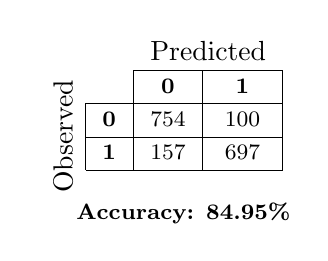
\begin{tikzpicture}
				\node[] at (0, 0) {
					\begin{tabular}{c|c|c|c|}
						\multicolumn{2}{c}{} & \multicolumn{2}{c}{\ticktitlesize{Predicted}} \\
						\cline{3-4}
						\multicolumn{1}{l}{\parbox[t]{2mm}{\multirow{4}{*}{\rotatebox[origin=c]{90}{\ticktitlesize{Observed}}}}} & \multicolumn{1}{c|}{} & \footnotesize{\textbf{0}} & \footnotesize{\textbf{1}} \\
						\cline{2-4}
						&\footnotesize{\textbf{0}}&\footnotesize{754}&\footnotesize{100}\\
						\cline{2-4}
						&\footnotesize{\textbf{1}}&\footnotesize{157}&\footnotesize{697}\\
						\cline{2-4}
					\end{tabular}
				};
				\node[] at (0.3, -1.4) {
					\textbf{\footnotesize{Accuracy: 84.95\%}}
				};
			\end{tikzpicture}
			\vspace*{0.89cm}
		\end{minipage}
		% No empty line here
		\begin{minipage}{0.6\textwidth}
			\newcommand{\marksize}{2pt}
			\begin{tikzpicture}
				\begin{axis}[
					height=0.5\textwidth,
					width=1.1\textwidth,
					xlabel=\ticktitlesize{Sample size},
					ylabel=\ticktitlesize{AUC},
					every tick label/.append style={font=\ticklabelsize},
					xmode=log,
					xmax=750,
					xtick={10, 30, 100, 300},
					xticklabels={10, 30, 100, 300},
					ymin=0.5,
					ymax=1,
					ytick pos=right,
					xtick pos=bottom,
					xtick style={draw=none},
					ytick style={draw=none},
					xmajorgrids=true,
					ymajorgrids=true,
					ytick={0.5, 0.6, 0.7, 0.8, 0.9, 1},
					y label style={at={(axis description cs:1.12,0.5)},anchor=north},
					clip=false
				]
					\addplot[only marks, fill=cb-green, mark size=\marksize] coordinates {
						(506, 0.942)
						(438, 0.850)
						(226, 0.900)
						(92, 0.906)
					};

					\addplot[only marks, fill=cb-light-purple, mark size=\marksize] coordinates {
						(290, 0.944)
						(74, 0.848)
						(38, 0.997)
						(22, 0.950)
						(12, 0.666)
						(10, 0.76)
					};
					\coordinate (legend) at (axis cs: 70, 0.45);
					\node[anchor=south] at (axis cs: 506, 0.942) {\textbf{\tiny{ADNI}}};
					\node[anchor=north] at (axis cs: 438, 0.850) {\textbf{\tiny{OASIS}}};
					\node[anchor=south] at (axis cs: 290, 0.944) {\textbf{\tiny{ADNI}}};
					\node[anchor=north] at (axis cs: 226, 0.900) {\textbf{\tiny{Oslo}}};
					\node[anchor=south] at (axis cs: 92, 0.906) {\textbf{\tiny{AIBL}}};
					\node[anchor=north] at (axis cs: 74, 0.848) {\textbf{\tiny{ANM}}};
					\node[anchor=north] at (axis cs: 38, 0.997) {\textbf{\tiny{MIRIAD}}};
					\node[anchor=east] at (axis cs: 22, 0.95) {\textbf{\tiny{AIBL}}};
					\node[anchor=north] at (axis cs: 12, 0.666) {\textbf{\tiny{OASIS}}};
					\node[anchor=south] at (axis cs: 10, 0.76) {\textbf{\tiny{ANM}}};
				\end{axis}
			\end{tikzpicture}
		\end{minipage}

	\end{frame}

	\begin{frame}{Layerwise Relevance Propagation}
		\centering
		\vfill
		\begin{tikzpicture}
			\node[] at (0, 0) {
				\includegraphics[width=3cm]{data/samples/subject1.png}
			};

			\node[] at (3.5, 0) {
				\includegraphics[width=3cm]{data/samples/subject2.png}
			};

			\node[] at (7, 0) {
				\includegraphics[width=3cm]{data/samples/subject3.png}
			};
		\end{tikzpicture}
		\vfill
	\end{frame}

	\begin{frame}{Validation}
		\centering
		\vfill
		\begin{tikzpicture}
			\node[] at (-2, -2) {};
			\node[] at (9, 2) {};
			\node[] at (0, 0) {
				\includegraphics[width=3cm]{data/averages/dementia.png}
			};
		\end{tikzpicture}
		\vfill
	\end{frame}

	\begin{frame}{Validation}
		\centering
		\vfill
		\begin{tikzpicture}
			\node[] at (-2, -2) {};
			\node[] at (9, 2) {};
			\node[] at (0, 0) {
				\includegraphics[width=3cm]{data/averages/dementia.png}
			};

			\node[] at (3.5, 0) {
				\includegraphics[width=3cm]{data/averages/ALE.png}
			};
		\end{tikzpicture}
		\vfill
	\end{frame}

	\begin{frame}{Validation}
		\centering
		\vfill
		\begin{tikzpicture}
			\node[] at (-2, -2) {};
			\node[] at (9, 2) {};
			\node[] at (0, 0) {
				\includegraphics[width=3cm]{data/averages/dementia.png}
			};

			\node[] at (3.5, 0) {
				\includegraphics[width=3cm]{data/averages/ALE.png}
			};

			\node[] at (7, 0) {
				\includegraphics[width=3cm]{data/overlap/test_90.png}
			};
		\end{tikzpicture}
		\vfill
	\end{frame}

	\begin{frame}{Validation} % Regions
		\newcommand{\annotation}[4]{
            \node[anchor=####4,align=center,font=\tiny\linespread{0.8}\selectfont,inner sep=2.5pt] at (axis cs: ####2,####3) {####1};
        }

		\centering
		\vfill
        \begin{tikzpicture}
            \begin{axis}[
                width=\textwidth,
                height=0.6\textwidth,
                ylabel=\footnotesize{ALE activation},
                xlabel=\footnotesize{LRP activation},
                ticks=none,
                xmin=0,
                xmax=1.25,
                ymin=0,
                ymax=1.1,
                axis y line=left,
                axis x line=bottom
            ]
                \addplot[only marks, fill=cb-light-purple, draw=black] table [col sep=comma, x=lrp, y=ale] {data/regions/test_mean.csv};
                \annotation{Left Accumbens}{0.906}{1}{south}
                \annotation{Right Accumbens}{0.731}{0.914}{north}
                \annotation{Left Amygdala}{1}{0.719}{south}
                \annotation{Right Amygdala}{0.767}{0.699}{north}
                \annotation{Parahippocampal\\Gyrus}{0.594}{0.415}{south}
                \annotation{Heschl's\\Gyrus}{0.785}{0.276}{south}
                \annotation{Lingual\\Gyrus}{0.517}{0.312}{north}
                \annotation{Planum\\Temporale}{0.407}{0.159}{north}
            \end{axis}
        \end{tikzpicture}
		\vfill
	\end{frame}

	\begin{frame}{Prognosis and personalization}
		\newcommand{\linestyle}{densely dotted}
        \newcommand{\diffx}{-7.05}
        \newcommand{\legendy}{0.92}

		\centering
		\vfill

        \begin{tikzpicture}
            \begin{axis}[
                height=0.6\textwidth,
                width=0.8\textwidth,
                xmin=-9,
                xmax=0,
                ymin=0,
                ymax=1,
                xlabel=\footnotesize{Years to diagnosis},
                ylabel=Group-wise mean\\dementia prediction,
                error bars/y dir=both,
                error bars/y explicit,
                every tick label/.append style={font=\scriptsize},
                ylabel style={align=center, font=\footnotesize\linespread{0.9}\selectfont}
            ]
                    \addplot[\linestyle] coordinates {
                        (-9, 0.309)
                        (0, 0.309)
                    } node [pos=0, anchor=north west] {\tiny{\textcolor{controls-default}{0.309}}};

                    \addplot[\linestyle] coordinates {
                        (-9, 0.656)
                        (0, 0.656)
                    } node [pos=0, anchor=south west] {\tiny{\textcolor{cases-default}{0.656}}};

                    \addplot[
                        cases-default,
                        scatter,
                        scatter/use mapped color={
                            draw=cases-default,
                            fill=cases-default
                        },
                        visualization depends on=\thisrow{declining_size}\as\size,
                        scatter/@pre marker code/.append style={
                            /tikz/mark size=\size ^ 0.3,
                            /tikz/mark color=cases-default
                        }
                    ] table [
                        col sep=comma,
                        x=year,
                        y=declining_mean,
                    ] {data/yearly_trajectories.csv};

                    \addplot[
                        controls-default,
                        scatter,
                        scatter/use mapped color={
                            draw=controls-default,
                            fill=controls-default
                        },
                        visualization depends on=\thisrow{declining_size}\as\size,
                        scatter/@pre marker code/.append style={
                            /tikz/mark size=\size ^ 0.3,
                            /tikz/mark color=cases-default
                        }
                    ] table [
                        col sep=comma,
                        x=year,
                        y=stable_mean,
                    ] {data/yearly_trajectories.csv};

                \node[anchor=west, align=left] at (axis cs: \diffx, 0.415) {\tiny{$\beta=0.44$}};
                \node[anchor=west, align=left] at (axis cs: \diffx, 0.385) {\tiny{$p=4.87 \times 10^{-60}$}};

                \draw[<->] (axis cs: \diffx, 0.309) -- (axis cs: \diffx, 0.656);
                \node[circle, minimum size=5.4pt, fill=gray, inner sep=0pt, anchor=north west] (n25mark) at (axis cs: -8.5, 0.9) {};

                \coordinate (label) at (axis cs: -11.37, 0.87);
            \end{axis}

            \node[anchor=west, inner sep=0pt] (n25label) at ($ (n25mark.east) + (0.05, 0) $) {\scriptsize{n=25}};
            \node[anchor=west, circle, minimum size=8.5pt, fill=gray, inner sep=0pt] (n100mark) at ($ (n25label.east) + (0.1, 0) $) {};
            \node[anchor=west, inner sep=0pt] (n100label) at ($ (n100mark.east) + (0.05, 0) $) {\scriptsize{100}};
            \node[anchor=west, circle, minimum size=12pt, fill=gray, inner sep=0pt] (n250mark) at ($ (n100label.east) + (0.1, 0) $) {};
            \node[anchor=west, inner sep=0pt] (n250label) at ($ (n250mark.east) + (0.05, 0) $) {\scriptsize{250}};
        \end{tikzpicture}
		\vfill
	\end{frame}

	\begin{frame}{Prognosis and personalization}
		\centering
		\vfill
		\begin{figure}
			\resizebox{0.9\textwidth}{!}{%
				\newcommand{\mriwidth}{2.59cm}
				\newcommand{\gap}{0.00cm}

				\colorlet{ninety}{cb-red-purple}
				\colorlet{fifty}{cb-blue}
				\colorlet{ten}{cb-green}

				\newsavebox{\first}
				\sbox{\first}{%
					\begin{tikzpicture}
						\begin{axis}[
							height=3cm,
							width=1.605 * \mriwidth,
							ylabel style={
								align=center,
								font=\scriptsize\linespread{0.8}\selectfont,
								at={(axis description cs:1.2,0.5)}
							},
							xlabel style={
								at={(axis description cs: 0.5, -0.2)}
							},
							ylabel={Healthy\\fraction},
							xlabel=\scriptsize{Age},
							every tick label/.append style={font=\tiny},
							xtick pos=bottom,
							ytick pos=right,
							ymin=0,
							ymax=1,
							xmin=62,
							xmax=95,
							ytick={0, 0.2, 0.4, 0.6, 0.8, 1.0},
							ytick style={draw=none},
							ymajorgrids=true,
							grid style={line width=.5pt, draw=gray!25},
						]

						\addplot[fifty, very thick] table [col sep=comma, x=age, y=baseline] {data/survival/survival_0.csv};
						\addplot[ten, very thick] table [col sep=comma, x=age, y=tenth] {data/survival/survival_0.csv};
						\addplot[ninety, very thick] table [col sep=comma, x=age, y=ninetyeth] {data/survival/survival_0.csv};
						\node[anchor=south west,font=\scriptsize] at (axis cs: 62, 0.3) {
							$\beta\mathrm{=}0.24$
						};
						\node[anchor=south west,font=\scriptsize] at (axis cs: 62, 0.1) {
							$p\mathrm{=}1.30*10^{-5}$
						};
						\end{axis}
					\end{tikzpicture}
					}

				\newsavebox{\second}
				\sbox{\second}{%
					\begin{tikzpicture}
						\begin{axis}[
							height=3cm,
							width=1.605 * \mriwidth,
							every tick label/.append style={font=\tiny},
							xtick pos=bottom,
							ytick pos=right,
							ymin=0,
							ymax=1,
							xmin=62,
							xmax=95,
							ytick={0, 0.2, 0.4, 0.6, 0.8, 1.0},
							yticklabels={,,},
							ytick style={draw=none},
							ymajorgrids=true,
							grid style={line width=.5pt, draw=gray!25},
						]

						\addplot[fifty, very thick] table [col sep=comma, x=age, y=baseline] {data/survival/survival_2.csv};
						\addplot[ten, very thick] table [col sep=comma, x=age, y=tenth] {data/survival/survival_2.csv};
						\addplot[ninety, very thick] table [col sep=comma, x=age, y=ninetyeth] {data/survival/survival_2.csv};
						\node[anchor=south west,font=\scriptsize] at (axis cs: 62, 0.3) {
							$\beta\mathrm{=}-0.19$
						};
						\node[anchor=south west,font=\scriptsize] at (axis cs: 62, 0.1) {
							$p\mathrm{=}1.24*10^{-16}$
						};
						\end{axis}
					\end{tikzpicture}
				}

				\newsavebox{\third}
				\sbox{\third}{%
					\begin{tikzpicture}
						\begin{axis}[
							height=3cm,
							width=1.605 * \mriwidth,
							every tick label/.append style={font=\tiny},
							xtick pos=bottom,
							ytick pos=right,
							ymin=0,
							ymax=1,
							xmin=62,
							xmax=95,
							ytick={0, 0.2, 0.4, 0.6, 0.8, 1.0},
							yticklabels={,,},
							ytick style={draw=none},
							ymajorgrids=true,
							grid style={line width=.5pt, draw=gray!25},
						]

						\addplot[fifty, very thick] table [col sep=comma, x=age, y=baseline] {data/survival/survival_3.csv};
						\addplot[ten, very thick] table [col sep=comma, x=age, y=tenth] {data/survival/survival_3.csv};
						\addplot[ninety, very thick] table [col sep=comma, x=age, y=ninetyeth] {data/survival/survival_3.csv};
						\node[anchor=south west,font=\scriptsize] at (axis cs: 62, 0.3) {
							$\beta\mathrm{=}-0.20$
						};
						\node[anchor=south west,font=\scriptsize] at (axis cs: 62, 0.1) {
							$p\mathrm{=}4.55*10^{-11}$
						};
						\end{axis}
					\end{tikzpicture}
				}

				\newcommand{\correlationplot}[4]{
					\begin{tikzpicture}
						\begin{axis}[
							height=1.58 * \mriwidth,
							width=1.605 * \mriwidth,
							xmajorticks=false,
							ylabel=####3,
							ytick={0, 1, 2, 3, 4, 5},
							yticklabels=####2,
							xmin=-1,
							xmax=17,
							ymin=0,
							ymax=6,
							every tick label/.append style={font=\tiny},
							ytick pos=left,
							scatter/classes={
								ADNI_EF={color0, draw=black},
								ADNI_MEM={color1, draw=black},
								CDCARE={color2, draw=black},
								CDCOMMUN={color3, draw=black},
								CDGLOBAL={color4, draw=black},
								CDHOME={color5, draw=black},
								CDJUDGE={color6, draw=black},
								CDMEMORY={color7, draw=black},
								CDORIENT={color8, draw=black},
								FAQTOTAL={color9, draw=black},
								GDTOTAL={color10, draw=black},
								MMSCORE={color11, draw=black},
								NPISCORE={color12, draw=black},
								PHC_EXF={color13, draw=black},
								PHC_LAN={color14, draw=black},
								PHC_MEM={color15, draw=black},
								PHC_VSP={color16, draw=black}
							},
							y label style={at={(-0.1,0.5)}},
							ymajorgrids=true,
							ytick style={draw=none}
						]
							\addplot[
								only marks,
								scatter,
								scatter src=explicit symbolic
							] table [
								col sep=comma,
								x=index,
								y=component_####1,
								meta=symptom
							] {data/correlations.csv};
							\addplot[dashed] coordinates {
								(-1, 2.85)
								(17, 2.85)
							};
							####4
						\end{axis}
					\end{tikzpicture}
				}

				\newsavebox{\firstcorrelations}
				\sbox{\firstcorrelations}{%
					\correlationplot{0}{{0, 1, 2, 3, 4, 5}}{\scriptsize{$-log_{10}(p)$}}{
						\node[] at (axis cs: 12.8, 3.65) {\tiny{PHC\_LAN}};
					}
				}
				\newsavebox{\secondcorrelations}
				\sbox{\secondcorrelations}{%
					\correlationplot{1}{{,,}}{{}}{
						\node[] at (axis cs: 11, 2.4) {\tiny{MMSCORE}};
						\node[] at (axis cs: 12, 3.35) {\tiny{NPISCORE}};
					}
				}
				\newsavebox{\thirdcorrelations}
				\sbox{\thirdcorrelations}{%
					\correlationplot{2}{{,,}}{{}}{
						\node[] at (axis cs: 4.4, 4.75) {\tiny{ADNI\_EF}};
						\node[] at (axis cs: 13, 5) {\tiny{PHC\_EXF}};
					}
				}
				\newsavebox{\fourthcorrelations}
				\sbox{\fourthcorrelations}{%
					\correlationplot{3}{{,,}}{{}}{}
				}

				\begin{tikzpicture}
					\node[] (first) at (0, 0) {
						\includegraphics[
							width=\mriwidth,
							clip=true,
							trim = 192mm 232mm 0mm 0mm
						]{data/components/component_0.png}
					};
					\node[anchor=north west] (first-survival) at ($ (first.south west) + (0, 0.35) $) {
						\usebox{\first}
					};
					\node[anchor=north west] (first-correlation) at ($ (first-survival.south west) + (-0.85, 0.25) $) {
						\usebox{\firstcorrelations}
					};

					\node[anchor=north east] at ($ (first.north west) - (0.07, 0.2) $) {{\Large{\textbf{c}}}};
					\node[anchor=north east] at ($ (first-survival.north west) - (0, 0.2) $) {{\Large{\textbf{d}}}};
					\node[anchor=north east] at ($ (first-correlation.north west) + (0.8, -0.2) $) {{\Large{\textbf{e}}}};

					\node[anchor=west] (second) at ($ (first.east) + (\gap, 0) $) {
						\includegraphics[
							width=\mriwidth,
							clip=true,
							trim = 192mm 232mm 0mm 0mm
						]{data/components/component_1.png}
					};
					\node[anchor=north west] (second-correlation) at ($ (first-correlation.north east) - (0.58, 0) $) {
						\usebox{\secondcorrelations}
					};

					\node[anchor=west] (third) at ($ (second.east) + (\gap, 0) $) {
						\includegraphics[
							width=\mriwidth,
							clip=true,
							trim = 192mm 232mm 0mm 0mm
						]{data/components/component_2.png}
					};
					\node[anchor=north west] (third-survival) at ($ (third.south west) + (0, 0.3) $) {
						\usebox{\second}
					};
					\node[anchor=north west] (third-correlation) at ($ (second-correlation.north east) - (0.58, 0) $) {
						\usebox{\thirdcorrelations}
					};

					\node[anchor=west] (fourth) at ($ (third.east) + (\gap, 0) $) {
						\includegraphics[
							width=\mriwidth,
							clip=true,
							trim = 192mm 232mm 0mm 0mm
						]{data/components/component_3.png}
					};
					\node[anchor=north west] (fourth-survival) at ($ (fourth.south west) + (0, 0.3) $) {
						\usebox{\third}
					};
					\node[anchor=north west] (fourth-correlation) at ($ (third-correlation.north east) - (0.58, 0) $) {
						\usebox{\fourthcorrelations}
					};

					\node[anchor=north east, inner sep=2pt] (legend-header) at ($ (third-survival.north west) - (0.22, 0.33) $) {\scriptsize{\underline{Percentiles}}};
					\node[anchor=north west, inner sep=1pt] (tenth) at ($ (legend-header.south east) - (0.83, 0) $) {\scriptsize{5th}};
					\node[anchor=north west, inner sep=1pt] (fiftieth) at (tenth.south west) {\scriptsize{50th}};
					\node[anchor=north west, inner sep=1pt] (ninetyeth) at (fiftieth.south west) {\scriptsize{95th}};
					\draw[draw=ten, very thick, text depth=0] ($ (tenth.west) + (-0.43, 0) $) -- ($ (tenth.west) + (-0.05, 0) $);
					\draw[draw=fifty, very thick, text depth=0] ($ (fiftieth.west) + (-0.43, 0) $) -- ($ (fiftieth.west) + (-0.05, 0) $);
					\draw[draw=ninety, very thick, text depth=0] ($ (ninetyeth.west) + (-0.43, 0) $) -- ($ (ninetyeth.west) + (-0.05, 0) $);
				\end{tikzpicture}

    		}%
		\end{figure}
		\vfill
	\end{frame}
\end{document}
